%%%%%%%%%%%%%%%%%%%%%%%%%%%%%%%%%%%%%%%%%%%%%%%%%%%%%%%
%                File: OpEx_style.tex                 %
%             Created: 2 September 2009               %
%                Updated: 15 May 2015                 %
%                                                     %
%           LaTeX template file for use with          %
%           OSA's journals Optics Express,            %
%             Biomedical Optics Express,              %
%            and Optical Materials Express            %
%                                                     %
%  send comments to Theresa Miller, tmiller@osa.org   %
%                                                     %
% This file requires style file, opex3.sty, under     %
%              the LaTeX article class                %
%                                                     %
%   \documentclass[10pt,letterpaper]{article}         %
%   \usepackage{opex3}                                %
%                                                     %
%                                                     %
%       (c) 2015 Optical Society of America           %
%%%%%%%%%%%%%%%%%%%%%%%%%%%%%%%%%%%%%%%%%%%%%%%%%%%%%%%

%%%%%%%%%%%%%%%%%%%%%%% preamble %%%%%%%%%%%%%%%%%%%%%%%%%%%
\documentclass[10pt,letterpaper]{article}
\usepackage{opex3}
\usepackage{color}
\usepackage{amsmath}
\usepackage{graphicx, subfigure}
\usepackage{threeparttable}
\usepackage{amsfonts}

%%%%%%%%%%%%%%%%%%%%%%% begin %%%%%%%%%%%%%%%%%%%%%%%%%%%%%%
\begin{document}

\title{Review of Quantitative Phase Imaging Microscopy (working title)}

\author{Manuel Bedrossian$^{1,*}$, J. Kent Wallace$^{2}$, Eugene Serabyn$^2$, and Jay Nadeau$^1$}

\address{$^1$Division of Aerospace Engineering, California Institute of Technology, 1200 E. California Blvd., Pasadena CA 91125, USA\\
$^2$Jet Propulsion Laboratory, California Institute of Technology, 4800 Oak Grove Dr., Pasadena, CA. 91109, USA}

\email{$^*$mbedross@caltech.edu} %% email address is required

% \homepage{http:...} %% author's URL, if desired

%%%%%%%%%%%%%%%%%%% abstract and OCIS codes %%%%%%%%%%%%%%%%
%% [use \begin{abstract*}...\end{abstract*} if exempt from copyright]

\begin{abstract}
This is a placeholder for the abstract. This section will be written as the contents and order of the paper are solidified.
\end{abstract}

\ocis{(000.0000) General.} % REPLACE WITH CORRECT OCIS CODES FOR YOUR ARTICLE, MINIMUM OF TWO; Avoid using the OCIS codes for “General” or “General science” whenever possible.
%For a complete list of OCIS codes, visit: http://www.opticsinfobase.org/submit/ocis/

%%%%%%%%%%%%%%%%%%%%%%% References %%%%%%%%%%%%%%%%%%%%%%%%%
\begin{thebibliography}{99}
\bibitem{bib1}P. J. Harshman, T. K. Gustafson, and P. Kelley, ``Title of paper," J. Chem. Phys. {\bf 3}, (to be published).

\bibitem{gallo99} K. Gallo and G. Assanto, ``All-optical diode based on second-harmonic generation in an asymmetric waveguide,'' \josab {\bf 16}(2), 267--269 (1999).

\bibitem{Masters98a} B. R. Masters, ``Three-dimensional microscopic tomographic imagings of the cataract in a human lens in vivo,'' \opex {\bf 3}(9), 332--338 (1998).

\bibitem{Oron03}

\bibitem{samplefig}
B.~N.~Behnken, G.~Karunasiri, D.~R.~Chamberlin, P.~R.~Robrish, and J.~Faist,
``Real-time imaging using a 2.8~THz quantum cascade laser and uncooled infrared microbolometer camera,''
\ol \textbf{33}(5), 440--442 (2008).

\end{thebibliography}

%%%%%%%%%%%%%%%%%%%%%%%%%%  body  %%%%%%%%%%%%%%%%%%%%%%%%%%
\section{Introduction}
Quantitative Phase Imaging (QPI) is becoming a prominant tool in the field of microscopy. 

\section{Theory}
QPI is most commonly performed by the use of optical interferometry. This technique encodes both the amplitude characteristics of an object as well as its phase characteristics. It does this with the help of a reference light beam that encodes the unaltered phase of the light before interacting with the sample.The reference beam and sample beam are recombined at the detector plane which then creates interference patterns, or an interferogram.The beams of an interferometer can be represented as waves of identical wavelengths, such that their displacement functions are:

\begin{subequations}
\begin{equation}
 \psi_1(x,y,t)=A_1(x,y)e^{i(\phi_1(x,y)-\omega t)}
 \end{equation}
 \begin{equation}
 \psi_2(x,y,t)=A_2(x,y)e^{i(\phi_2(x,y)-\omega t)}
 \end{equation}
 \end{subequations}
 
 Where $A_1$ and $A_2$ are the amplitudes of the electric field as a function of $x$ and $y$, $\phi_1$ and $\phi_2$ are relative phases of waves 1 and 2 respectively, and $\omega$ is the angular frequency of the wave. 
 
 The combination of these two waves at the detector plane causes the resultant wave to be expressed using the superposition principle such that:
 
 \begin{equation}
 \Psi(x,y,t)=\psi_1+\psi_2=A_1(x,y)e^{i(\phi_1(x,y)-\omega t)}+A_2(x,y)e^{i(\phi_2(x,y)-\omega t)}
 \end{equation}
 
 Modern optical detector arrays, as capable as they are, cannot distinguish wavelengths of light. Their mode of operation is by the integration of the light incident on it for a certain period of time, often called the integration time or shutter speed. The measured electric field by the detector becomes:
 
 \begin{equation}
 I(x,y)=\int_{t_1}^{t_2}\Psi \Psi^*dt=I_1+I_2+2\sqrt{I_1I_2}\cos(\phi_1-\phi_2)
 \label{eq:intensity}
 \end{equation}
 
 Where $\Psi^*$ is the complex conjugate of $\Psi$, and $I_1$ and $I_2$ are the intensities of beams $1$ and $2$, respectively.
 
 A common algorithm for the extraction of quantitative phase information from such interferograms, or fringes, is called the `Four Step' or `Four Bucket' Method, where at least four samples must be made per fringe. Figure \ref{fig:fringe} shows a fringe that has been sampled at the four points marked by asterisks.
 
 \begin{figure}
 \centering
 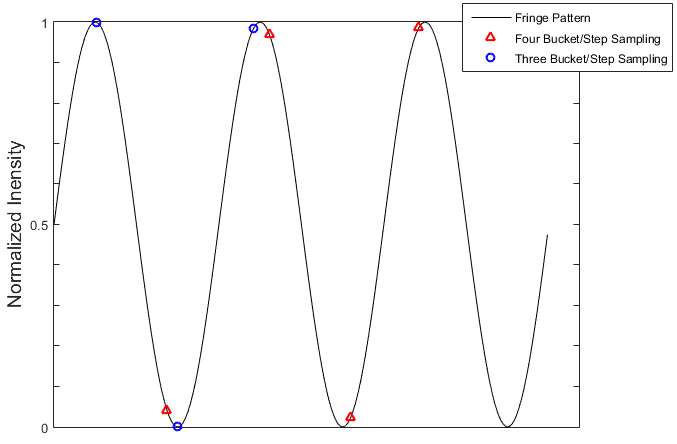
\includegraphics[width=0.8\linewidth]{fringe.png}
 \caption{A fringe that has been sampled at four discrete points}
 \label{fig:fringe}
 \end{figure}
 
 According to Equation \ref{eq:intensity}, the intensities of the electric field at each of the four sample points are:
 
 \begin{subequations}
 \begin{equation}
 I_a=I_1+I_2+2\sqrt{I_1I_2}\cos\phi
 \end{equation}
 \begin{equation}
 I_b=I_1+I_2+2\sqrt{I_1I_2}\cos(\phi+\pi/2)=I_1+I_2-2\sqrt{I_1I_2}\sin\phi
 \end{equation}
 \begin{equation}
 I_c=I_1+I_2+2\sqrt{I_1I_2}\cos(\phi+\pi)=I_1+I_2-2\sqrt{I_1I_2}\cos\phi
 \end{equation}
 \begin{equation}
 I_d=I_1+I_2+2\sqrt{I_1I_2}\cos(\phi+3\pi/2)=I_1+I_2+2\sqrt{I_1I_2}\sin\phi
 \end{equation}
 \end{subequations}
 
 With these equations describing the electric fields of the incident light, the phase difference between the two beams of light ($\phi$) becomes:
 
 \begin{equation}
\phi=\arctan\left(\frac{\sin\phi}{\cos\phi}\right)=\arctan\left(\frac{I_d-I_b}{I_a-I_c}\right) 
\end{equation}

\subsection{Phase Unwrapping}

Due to angles' cyclic nature, phase values obtained from interferometric techniques are bounded between $[0,\pi]$ or $[0,2\pi]$. This gives rise to discontinuities in phase calculations from interferometric techniques.

\begin{figure}
\centering
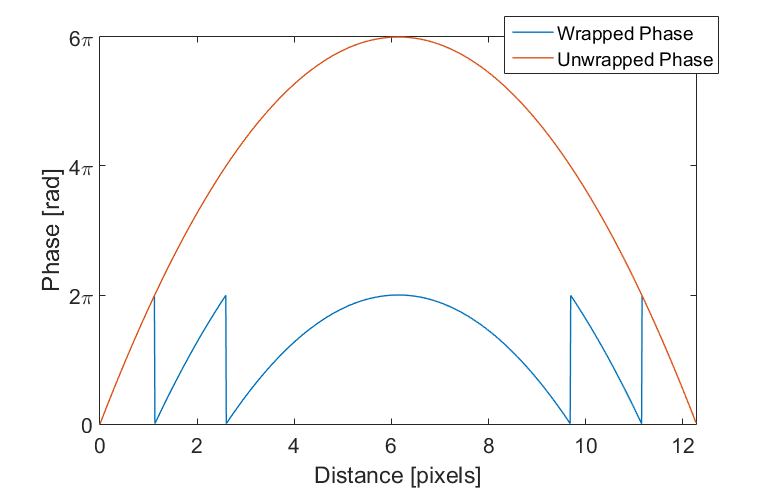
\includegraphics[width=0.8\textwidth]{phaseUnwrapped.png}
\caption{Wrapped and unwrapped computer simulated phase profiles}
\label{fig:phaseUN}
\end{figure}

Figure \ref{fig:phaseWrap} shows a computer simulated phase profile that ranges from $[0,2\pi]$. In this figure we can see discontinuities in the phase profile as it jumps from $2\pi$ to $0$ and vice versa. In Figure \ref{fig:phaseUN}, the same phase profile is shown after unwrapping.

\section{QPI Instrumentation}

 Interference patterns can be caused by one of many ways. The fundamental concept behind fringe creation is a difference in path length between the two beams. This difference in path length can be caused by requiring one beam of light to physically travel further than the other, or by delaying one beam by having it pass through an object with a different index of refraction than the other beam.
 
 There are many experimental setups that can create these necessary interference patterns with which amplitude and phase information can be analyzed. These setups include, but are not limited to, the Michelson, Mach-Zehnder, Fizeau, and the Fabry P\'{e}rot interferometers. Figure \ref{fig:types} shows optical schematics of each of these interferometers.
 
 \begin{figure}
 \centering
 \subfigure[Michelson Interferometer]{\includegraphics[width=0.45\textwidth]{Michellson1.png}}
 \subfigure[Mach-Zehnder Interferometer]{\includegraphics[width=0.45\textwidth]{Mach-Zehnder1.png}}
 \subfigure[Fabry-P\'{e}rot interferometer]{\includegraphics[width=0.6\textwidth]{Fabry-Perot1.png}}
 \label{fig:types}
 \caption{Various interferometer types}
 \end{figure}
 
 \subsection{Holography}
 
 Holography is a subset of interferometry and is used to record the interferogram, or hologram on a detector plane, without the use of a lens or other optical components to produce an image first. There are three major types of holography: in-line, twin-beam, and off-axis holography. Due to the advancements in detector array capabilities, sizes, and reductions in cost, Digital Holographic Micrscopy (DHM) is becoming a useful tool in microscopy.
 
 \subsubsection{In-Line Holography}
 
 In-line holography is a single beam holographic setup. A single coherent light source is used to illuminate a sample of interest. The coherent light interacts with the sample by being absorbed and/or diffracted. The light interactions are recorded at a detector plane, which captures the samples three-dimensional morphology. Because this method does not use a reference beam, quantitative phase is not possible with this method, although it was reported by (***INSERT CITATION***) that phase \textit{contrast} microscopy is possible by obtaining out of focus in-line holographic images.
 
 \subsubsection{Twin-Beam Holography}
 \subsubsection{Off-Axis Holography}
 
 Off-axis Digital Holographic Microscopy (DHM) is becoming prominent in the microscopy community due to its ability to perform both intensity and quantitative phase measurements of a sample, perform these measurements of a three dimensional volume, and obtain all this information in a single image frame. Obtaining three spatial dimensions in a single two dimensional image allows the opportunity to acquire image sequences, which effectively yields four dimensional data ($x,y,z,t$) in both intensity and phase. In order to `decompress' the three dimensional information that has been encoded into a single hologram, a numerical reconstruction process is necessary.
 
 Numerical reconstruction, re-propagates the electric field encoded in the hologram to a desired focal point. This is accomplished by the convolution of the hologram with an electric field propagation term at the desired focal point, shown in Equation \ref{eq:recon}.(***INSERT CITATION***)
 
 \begin{equation}
 \Gamma(\xi,\eta)=\mathfrak{F}^{-1}[\mathfrak{F}(h\cdot R)*G]
 \label{eq:recon}
 \end{equation}
 
 Where $\Gamma(\xi,\eta)$ is the complex wavefront at the desired focus distance, $h$ is the hologram, $G$ is the electric field propagation term, and $\mathfrak{F}$ is the Fourier Transform operator. $R$ is a `phase adjustment' term that is used to remove tilt and other unwanted artifacts from the phase reconstructions. For this rest of this work, the phase adjustment term will be assumed to be unity as phase adjustments can also be made after the reconstruction process.
 
  The value and form of the propagation term $G$ depends on the optical setup of the DHM instrument but is always a complex function with a magnitude of unity. This adds no intensity to the hologram reconstruction, only provides phase information for the back propagation of the electric field. An example propagation term is shown in Equation \ref{eq:propa}.
 
 \begin{equation}
 G(m,n)=\exp\left[\frac{-2\pi di}{\lambda}\sqrt{1-\frac{\lambda^2\left(n+\frac{N_x^2\Delta x^2}{2d\lambda}\right)}{N_x^2\Delta x^2} - \frac{\lambda^2\left(m+\frac{N_y^2\Delta y^2}{2d\lambda}\right)}{N_y^2\Delta y^2}  }\right]
 \label{eq:propa}
 \end{equation}
 
 Where $d$ is the desired focus distance to be reconstructed, $\lambda$ is the wavelength of the illuminating light source, $N_x$ and $N_y$ are the pixel sizes of the detector in the $x$ and $y$ directions, and $\Delta x$ and $\Delta y$ are the pixel sizes in the $x$ and $y$ directions, respectively.
 
 The magnitude of $\Gamma(\xi,\eta)$ is the instensity of the incident light at the desired focus distance and the quantitative phase at the desired focus distance is:
 
 \begin{equation}
 \phi=\arctan\left(\frac{\mathfrak{Im}(\Gamma)}{\mathfrak{Re}(\Gamma)}\right)
 \end{equation}
 
 Where $\mathfrak{Im}(\Gamma)$ and $\mathfrak{Re}(\Gamma)$ are the imaginary and real components of $\Gamma$, respectively.
 
\section{Phase Errors and Noise}

As with any measurement, there are errors and noise that must be accounted for in the application of quanititative phase imaging.

\section{Abstract}
The abstract should be limited to approximately 100 words. It should be an explicit summary of the paper that states the problem, the methods used, and the major results and conclusions. It also should contain the relevant key words that would allow it to be found in a cursory computerized search. If the work of another author is cited in the abstract, that citation should be written out without a number, [e.g., journal, volume, first page, and year (Opt. Express {\bf 22}, 1234 (2014))], and a separate citation should be included in the body of the text. The first reference cited in the main text must be [1]. Do not include numbers, bullets, or lists inside the abstract.

\section{Figures, tables, and supplemental materials}

\subsection{Figures and tables}

OSA express journals encourage authors to submit color and multimedia figures with their manuscripts. Figures and tables should be placed in the body of the manuscript.

\begin{figure}[h]
\centering\includegraphics[width=7cm]{opexfig1}
\caption{Sample caption (Ref. \cite{Oron03}, Fig. 2).}
\end{figure}

\noindent Standard \LaTeX{} environments should be used to place tables and figures:
\begin{verbatim}
\begin{figure}[htbp]
\centering\includegraphics[width=7cm]{opexfig1}
\caption{Sample caption (Ref. \cite{Oron03}, Fig. 2).}
\end{figure}
\end{verbatim}

\subsection{Supplementary materials in OSA express journals}

Most OSA journals allow authors to include supplementary materials as integral parts of a manuscript. Such materials are subject to the same editorial standards and peer review procedures along with the rest of the paper and should be uploaded and described using OSA’s Prism manuscript system.

Authors can submit appropriate visualizations or small data files (see details below) for OSA to host. Large datasets and code or simulation files can be included but must be placed in an appropriate archival repository and cited as described here. 

\begin{table}[h]
\centering
\begin{threeparttable} 
\caption{Supplementary Materials Supported in OSA Journals$^a$}
\begin{tabular}{|l|l|}
\hline
Visualization & 2D image, 3D image, video \\ \hline
Data File     & Small data file such as data underlying a plot in a figure \\ \hline
Dataset       & Dataset stored in an appropriate external repository \\ \hline
Code          & Code or simulation files stored in an appropriate external repository \\
\hline
\end{tabular}
\begin{tablenotes}
\item [] $^a$\textit{Optica} allows authors to include a supplemental document that can contain additional text, equations, citations, etc. (see Supplementary Materials in \textit{Optica} for details, \url{https://www.osapublishing.org/submit/style/supplementary-materials-optica.cfm}). For all other OSA journals, supplemental text must be included as appendices within the primary manuscript.
\end{tablenotes}
\end{threeparttable} 
\end{table}

Video visualizations (formerly media files) are the most commonly submitted type of supplementary materials for the express journals. They typically illustrate a synopsis of research results. They are integral and as such should be included only when they convey essential information beyond what can be presented within the article's PDF representation. Video visualizations should be uploaded upon submission and peer-reviewed along with the manuscript. Video files must use open compression standards for display on broadly available applications such as VLC, Apple QuickTime, or Windows Media Player. MOV, AVI, MPG, and MP4 video containers are accepted. The following video guidelines will help with the submission process:

\begin{itemize}
\item 15 MB is the recommended maximum video file size.
\item 720 x 480 pixels (width by height) is the recommended screen size.
\item If appropriate, insert a representative frame from the video in the manuscript as a figure.
\item Minimize file size by using an acceptable codec such as QuickTime, x264, or XviD. HandBrake is an open source tool for converting video to common codecs. 
\item Videos must be playable on all platforms using QuickTime or VLC.
\item Animations must be formatted into a standard video container.
\end{itemize}

Visualizations must be associated with a figure, table, or equation OR be referenced in the results section of the manuscript. Use the label 11Visualization" and the item number to identify the visualization. Please note that to create text color for supplementary materials links, use of the color.sty package and the command \verb|\textcolor{blue}{Visualization}| is preferred to using the command \verb|\url{Visualization}|.

\newpage

\begin{figure}[h]
\centering\includegraphics{opexfig2}
\caption{Three traps create three rings of magnetic nanoparticles. The rings interact with one another (see \textcolor{blue}{Visualization 3}). [From Masajada et al., Opt. Lett. 38, 3910 (2013).]}
\end{figure}

\begin{verbatim}
\begin{figure}[h]
\centering\includegraphics{opexfig2}
\caption{Three traps create three rings of magnetic 
nanoparticles. The rings interact with one another (see 
\textcolor{blue}{Visualization 3}). [From Masajada 
et al., Opt. Lett. 38, 3910 (2013).]}
\end{figure}
\end{verbatim}

Please refer to the Author Guidelines for Supplementary Materials (\mbox{\url{http://www.osapublishing.org/submit/style/multimedia.cfm}}) for more detailed instructions on acceptable multimedia formats for audio and tabular data.


\section{Mathematical and scientific notation}

\subsection{Displayed equations} Displayed equations should be centered.
Equation numbers should appear at the right-hand margin, in
parentheses:
\begin{equation}
H = \frac{1}{2m}(p_x^2 + p_y^2) + \frac{1}{2} M{\Omega}^2
     (x^2 + y^2) + \omega (x p_y - y p_x).
\end{equation}

All equations should be numbered in the order in which they appear
and should be referenced  from within the main text as Eq. (1),
Eq. (2), and so on [or as inequality (1), etc., as appropriate].

\subsection{Inline math} To help with conversion, place all math in a proper math environment. For example, expression \mbox{$3\times 4 = 12$} should be set this way, \texttt{\$3$\backslash$times 4=12\$}, not this way, \texttt{3 \$$\backslash$times\$4=12}. Simple fractions for inline math
should use parentheses when necessary to avoid ambiguity, for
example, to distinguish between $1/(n-1)$ and $1/n-1$.  Exceptions
to this are the proper fractions such as $\frac{1}{2}$, which are
better left in this form. Summations and integrals that appear
within text such as $\frac{1}{2}{\sum }_{n=1}^{n=\infty} (n^2 -
2n)^{-1}$ should have limits placed to the right of the symbol to
reduce white space.

\subsection{General guidelines on notation} Notation must be
legible, clear, compact, and consistent with standard usage. In
general, acronyms should be defined at first use. Adherence to the
following guidelines will greatly assist the production process:

\paragraph*{\bf Radical signs.}
When possible, avoid oversized radical signs
by using the notation of a superscript $1/2$. For example, change
$\sqrt{(a + b)(a - c)}$ to $[(a + b)(a - c)]^{1/2}$.

\paragraph*{\bf Exponentials.} Avoid tiny superscripts of exponential $e$ (e.g.,
$e^{jkl})$ by using the alternative \verb+\exp+ notation,
$\exp(jkl)$.

\paragraph*{\bf Variables and vectors.}
Set single-letter variables in italics $(k)$. Set three-vectors in
boldface $(\mathbf{k})$. Functions, derivative ``d,''
abbreviations, and multiletter identifiers should be set in roman
(plain) type  ($\alpha \cos, \int\!\dots{\rm d}x, k^{\rm out}$).

\paragraph*{\bf Multiplication.}
In general, close up multiplied terms $(p_yp_x)$;
use $\times$ if multiplication sign is essential $(2 \times
10^{-2})$ or for continuation in displayed equations. Use raised dot only for scalar product $(\mathbf{k \cdot k})$.

\paragraph*{\bf Fences.}
For simple bracketing the usual order of parentheses and brackets
is $\{ \, [  \, (  \,  \{  \, [  \, (  \, |  \, )  \, ]  \, \} \,
)  \, ]  \, \}$.


\paragraph*{\bf Metric system.}
The metric system is used in OSA journals. If nonmetric units are
essential (e.g., for parts specifications), conversion should be
given at first mention:  ``. . . a $\frac{1}{4}$\,-in. bolt \mbox{(1 in.
= 2.54 cm).''}

\subsection{Acknowledgments} Acknowledgments, if included, should
appear at the end of the document, just before the references. The
number of a grant or contract should be omitted unless its
inclusion is required by the agency supporting the research. Use
the command \verb+\section*{Acknowledgments}+  to create a
nonnumbered section heading.

\section{References}
\label{sec:refs}
Proper formatting of references is extremely important, not only for consistent appearance but also for accurate electronic tagging. Please follow the guidelines provided below on formatting, callouts, and use of Bib\TeX.

\subsection{Formatting reference items}
Each source must have its own reference number. Footnotes (notes at the bottom of text pages) are not used in OSA journals. References require all author names, full titles, and inclusive pagination. Here are some examples of how to set the most common reference types:

\begin{description}
\item[Journal paper] \hfill\\
{\it Do not include web addresses in journal citations.}

C. van Trigt, ``Visual system-response functions and estimating reflectance,'' %\josaa
   J. Opt. Soc. Am. A {\bf 14}(4), 741--755 (1997).

S. Yerolatsitis, I. Gris-S\'anchez, and T. A. Birks,
``Adiabatically-tapered fiber mode multiplexers,'' Opt. Express {\bf 22}(1), 608--617 (2014).

\item[Journal paper identified by paper number] \hfill\\
{\it The paper number is sufficient. There is no need to give the number of pages.}

L. Rippe, B. Julsgaard, A. Walther, Y. Ying, and S. Kr\"oll,
``Experimental quantum-state tomography of a solid-state qubit,'' Phys. Rev. A {\bf 77}, 022307 (2008).

\item[Book] \hfill\\
T. Masters, {\it Practical Neural Network Recipes in C++} (Academic, 1993).

F. Ladouceur and J. D. Love, \textit{Silica-Based Buried Channel Waveguides and Devices} (Chapman \& Hall, 1995), Chap. 8.

\item[Article in a book] \hfill\\
D. F. Edwards, ``Silicon (Si),'' in {\it Handbook of Optical Constants of Solids,} E. D. Palik, ed. (Academic, 1985).

\item[Paper in a published conference proceedings] \hfill\\
R. E. Kalman, ``Algebraic aspects of the generalized inverse of a
rectangular matrix,'' in {\it Proceedings of Advanced Seminar on
Generalized Inverse and Applications,} M. Z. Nashed, ed. (Academic, 1976), pp. 111--124.

\item[Paper published in an OSA conference proceedings] \hfill\\
R. Craig and B. Gignac, ``High-power 980-nm pump lasers,'' in
{\it Optical Fiber Communication Conference}, Vol. 2 of 1996 OSA Technical Digest Series
(Optical Society of America, 1996), paper ThG1.

\item[Paper presented at a meeting/from an unpublished conference proceeding] \hfill\\
D. Steup and J. Weinzierl, ``Resonant THz-meshes,'' presented at the
Fourth International Workshop on THz Electronics,
Erlangen-Tennenlohe, Germany, 5--6 Sept. 1996.

\item[SPIE proceedings] \hfill\\
S. K. Griebel, M. Richardson, K. E. Devenport, and H. S. Hinton,
``Experimental performance of an ATM-based buffered hyperplane
CMOS-SEED smart pixel array,'' Proc. SPIE {\bf 3005}, 254--256 (1997).

{\it For later SPIE proceedings with a paper number, cite just the number and not any page information.}

S. Gu, F. Shao, G. Jiang, F. Li, and M. Yu,
``An objective visibility threshold measurement method for asymmetric stereoscopic images,''
Proc. SPIE {\bf 8205}, 820505 (2011).

\item[IEEE proceedings] \hfill\\
T. Darrel and K. Wohn, ``Pyramid based depth from focus,'' in
{\it Proceedings of IEEE Conference on Computer Vision and Pattern
Recognition} (IEEE, 1988), pp. 504--509.

\item[Paper accepted for publication] \hfill\\
D. Piao, ``Cancelation of coherent artifacts in optical coherence tomography imaging,'' Appl. Opt. (to be published).

D. W. Diehl and T. D. Visser,
"Phase singularities of the longitudinal field components in the focal region of a high-aperture optical system,"
J. Opt. Soc. Am. A, doc. ID 56789 (posted 11 November 2005, in press).

\item[Manuscript in preparation] \hfill\\
J. Q. Smith, Laboratory for Laser Energetics, University of Rochester, 250 East River Road, Rochester, New York 14623, USA, and K. Marshall are preparing a manuscript to be called ``Optical aspects in liquid crystals.''

\item[Personal communication] \hfill\\
T. Miller, Publications Department, Optical Society of
America, 2010 Massa\-chusetts Avenue, N.W., Washington, D.C.,
20036 (personal communication, 2010).

\item[Internet links] \hfill\\
Extreme Networks white paper, ``Virtual metropolitan area networks,'' (Extreme Networks, 2001), \texttt{http://www.extremenetworks.com/technology/
whitepapers/vMAN.asp}.

A. G. Ramm, ``Invisible obstacles,'' \texttt{http://www.arxiv.org/abs/math-ph
/0608034}.

\end{description}

The commands \verb+\begin{thebibliography}{}+ and \verb+\end{thebibliography}+ format the section according to standard style, showing the title {\bf References and links}.  Use the \verb+\bibitem{label}+ command to start each reference.

\subsection{Formatting reference citations}
References should be numbered consecutively in the order in which they are referenced in the body of the paper. Set reference callouts with standard \verb+\cite{}+ command or set manually inside square brackets [1].

To reference multiple articles at once, simply use the cite command with a comma separating the reference labels, e.g. \verb+\cite{gallo99,Masters98a,Oron03}+, produces \cite{gallo99,Masters98a,Oron03}. Using the \texttt{cite.sty} package will make these citations appear like so: [2--4].

\subsection{Bib\TeX}
\label{sec:bibtex}
Bib\TeX{} may be used to create a file containing the references, whose contents (i.e., contents of \texttt{.bbl} file) can then be pasted into the bibliography section of the \texttt{.tex} file. A new Bib\TeX{} style file, \texttt{osajnl.bst}, is provided.

To assist authors with journal abbreviations in references, standard abbreviations for 31 commonly cited journals have been included as macros within opex3.sty.  The abbreviations are shown in Table 1.

\begin{table}[htbp]
\centering\caption{Standard abbreviations
 for commonly cited journals.}
\begin{tabular}{lp{1.7in}|lp{1.7in}}
\hline
Macro        & Abbreviation                & Macro        & Abbreviation          \\ \hline
\verb+\ao+   & Appl.\  Opt.\               & \verb+\jpp+  & J. Phys.              \\
\verb+\aop+  & Adv. Opt. Photon.           & \verb+\nat+  & Nature                \\
\verb+\ap+   & Appl.\  Phys.\              & \verb+\oc+   & Opt.\ Commun.\        \\
\verb+\apl+  & Appl.\ Phys.\ Lett.\        & \verb+\opex+ & Opt.\ Express         \\
\verb+\apj+  & Astrophys.\ J.\             & \verb+\ol+   & Opt.\ Lett.\          \\
\verb+\bell+ & Bell Syst.\ Tech.\ J.\      & \verb+\ome+  & Opt.\ Mater.\ Express \\
\verb+\boe+  & Biomed.\ Opt.\ Express      & \verb+\opn+  & Opt.\ Photon.\ News   \\
\verb+\jqe+ & IEEE J.\ Quantum Electron.\  & \verb+\pl+   & Phys.\ Lett.\         \\
\verb+\assp+ & IEEE Trans.\ Acoust.\ Speech Signal Process.\  & \verb+\pr+ & Photon.\ Res.\ \\
\verb+\aprop+ & IEEE Trans.\  Antennas Propag.\    & \verb+\pra+ & Phys.\ Rev.\ A   \\
\verb+\mtt+ & IEEE Trans.\ Microwave Theory Tech.\ & \verb+\prb+ & Phys.\ Rev.\ B   \\
\verb+\iovs+ & Invest.\ Ophthalmol.\ Vis.\ Sci.\    & \verb+\prc+ & Phys.\ Rev.\ C   \\
\verb+\jcp+ & J.\ Chem.\ Phys.\            & \verb+\prd+ & Phys.\ Rev.\ D   \\
\verb+\jmo+ & J.\ Mod.\ Opt.\              & \verb+\pre+ & Phys.\ Rev.\ E   \\
\verb+\jocn+ & J.\ Opt.\ Commun.\ Netw.\   & \verb+\prl+ & Phys.\ Rev.\ Lett.\    \\
\verb+\jon+ & J.\ Opt.\ Netw.\             & \verb+\rmp+ & Rev.\ Mod.\ Phys.\    \\
\verb+\josa+ & J.\ Opt.\ Soc.\ Am.\        & \verb+\pspie+ & Proc.\ Soc.\ Photo-Opt.\ Instrum.\ Eng.\   \\
\verb+\josaa+ & J.\ Opt.\ Soc.\ Am.\ A     & \verb+\sjqe+ & Sov.\ J.\ Quantum Electron.\   \\
\verb+\josab+ & J.\ Opt.\ Soc.\ Am.\ B     & \verb+\vr+ & Vision Res.\   \\ \hline
\end{tabular}
\end{table}


\section{Conclusion}
After proofreading the manuscript, compress your .TEX manuscript file and all figures (which should be in EPS format, or PDF format if you are using PDF-\LaTeX) in a ZIP, TAR or TAR-GZIP package. Prism, OSA’s article tracking system, will process in \LaTeX mode by default but will use PDF-\LaTeX if PDF figure files are detected. Note: TAR or TAR-GZIP is no longer required. All files must be referenced at the root level (e.g., file \texttt{figure-1.eps}, not \texttt{/myfigs/figure-1.eps}). If there is video or other supplementary materials, the associated files should be uploaded separately.

\end{document}
